\documentclass[10pt,a4paper]{article}
\usepackage[utf8]{inputenc}
\usepackage[italian]{babel}
\usepackage{amsmath}
\usepackage{amsfonts}
\usepackage{amssymb}
\usepackage{graphicx}
\usepackage[left=2cm,right=2cm,top=2cm,bottom=2cm]{geometry}
\newcommand{\rem}[1]{[\emph{#1}]}

\author{Gruppo AC \\ Federico Belliardo, Giulia Franchi, Francesco Mazzoncini}
\title{Esercitazione N.6: Amplificatore operazionale: circuiti lineari}
\begin{document}
\section{Scopo dell'esperienza}

Misurare le caratteristiche di amplificatori invertenti e non invertenti realizzati con un op-amp TL081 in fig.\ref{pin}.
\begin{figure}[!htb]
  \centering
  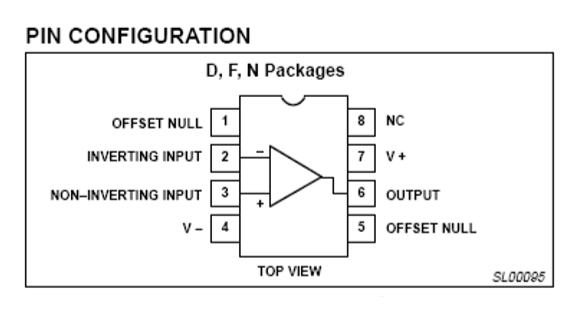
\includegraphics[scale=0.3]{pinrelaz6.png}
\caption{configurazione pin.}
\label{pin}
\end{figure}

\section{Amplificatore invertente}
\subsection{Realizzazione circuito}
\subsection{Misura del guadagno a frequenza fissata}
\subsection{Misura dell'impedenza d'ingresso}
\section{Risposta in frequenza del circuito e slew rate}
\subsection{Misura della risposta in frequenza}
\subsection{Slew rate}
\section{Amplificatore non invertente}
\end{document}